\section{Implementação de Software}

A implementação do software seguiu a estratégia de se implementar primeiramente componentes que não possuem dependência para funcionar, seguindo para os componentes que tem como dependência os que foram implementados e assim por diante. De forma geral, foi seguido o diagrama de componentes da figura \ref{fig:diagrama_componentes} no sentido da direita para esquerda, sendo implementadas em ordem: as camadas de banco de dados, de Negócio, Intermediária e de Interface. 


Além disso, foram priorizados serviços essenciais para o funcionamento geral do projeto, i.e., os componentes de Aplicação Mobile e Autenticação, que garantem melhoras na utilização do usuário e segurança da informação, foram considerados menos prioritários que os demais componentes, que atuam desempenham a função primária do projeto, que é controlar e monitorar a temperatura de fermentação de cervejas.


Os links de acesso para os repositórios de código fonte por componente são listados no apêndice \ref{appendice:repositorios}. Eles foram salvos na plataforma Github e serão mantidos públicos para consulta e oportunidade de continuidade do projeto, desde que seguindo os termos de licença especificados em cada repositório.


\subsection{Camada de Persistência}


A Camada de Persistência foi rapidamente implementada instanciando-se um banco de dados na nuvem da Amazon Web Services (AWS) pelo serviço RDS e executando o script de DDL (Data Definition Language) que foi gerado a partir do diagrama da figura \ref{fig:diagrama_entidade_relacionamento}. A plataforma utilizada para confecionar o diagrama (\url{https://dbdiagram.io/}) oferece o download do código de geração do banco de dados a partir do diagrama. Foram então realizadas algumas modificações no script gerado, para incluir a criação de índices e estabelecer o relacionamento entre as tabelas. O arquivo de extensão \textit{sql} para configuração do banco de dados está disponível no seguinte repositório de código: \url{https://github.com/josehcls/tcc-config}. O banco de dados foi provisionado pela plataforma de cloud computing AWS (Amazon Web Services)  


\subsection{Camada de Negócio}


\subsubsection{Servidores de Registro e Receitas}


Após a configuração do banco de dados, foram implementados os componentes responsáveis por transacionar os registros de Usuários, Dispositivos, Receitas, Lotes e Perfis de Controle. 
Os servidores de Registro (\url{https://github.com/josehcls/tcc-register-service}) e Receitas (\url{https://github.com/josehcls/tcc-recipe-service}) foram desenvolvidos na linguagem Java e desempenham as funções básicas de transação de dados: listagem, criação, atualização e deleção. 


O framework Spring foi utilizado para prover uma interface de programação REST, que serve de ponto de comunicação com o Servidor de Aplicação, ou API Gateway do projeto. Os servidores recebem solicitações de transação por meio dessa interface, realizam validações de consistências de dados e realizam as transações por meio de conexão direta ao banco de dados. Para validar as operações, foram criados testes automatizados durante o desenvolvimento, que podem ser executados para verificar a eficácia de cada um dos métodos implementados.


Após a implementação e testes gerais, foi confecionado o arquivo Dockerfile para configurar a geração de um container Docker a partir do pacote jar (Java Archive), resultado da compilação de cada um dos componentes.
Esse container é utilizado para simplificar e otimizar a implantação desses componentes, de forma a permitir o provisionamento de uma instância do serviço em nuvem com facilidade e celeridade.


\subsubsection{Servidor de Processamento}


O Servidor de Processamento (\url{https://github.com/josehcls/tcc-processor}) foi desenvolvido para receber as mensagens enviadas pelo Dispositivo com os dados coletados, processá-las e salvar as informações no banco de dados. Ele foi implementado na linguagem Python utilizando a biblioteca paho-mqtt, o programa se inscreve no tópico de mensagens MQTT para qual o Dispositivo publica as mensagens, e um código de tratamento é acionado a cada nova mensagem recebida. 


Na escala de um Dispositivo em operação, não se notou atraso significativo entre o recebimento da mensagem e disponibilização das informações no banco de dados, porém, uma possível melhoria desse sistema seria inserir a mensagem recebida em uma fila de processamento, utilizando softwares como o RabbitMQ, que então seria processada. Essa melhoria garantiria a retenção de mensagens em casos de queda do banco de dados e evitaria que o processamento e transação no banco de dados, que são as ações mais custosas desse fluxo, se sobrecarreguem e criem gargalos.


\subsubsection{Servidor de Análises}


Com a função de extrair e preparar as informações coletadas durante a fermentação para o usuário, foi implementada o Servidor de Análises (\url{https://github.com/josehcls/tcc-analytics}) utilizando a linguagem Python em conjunto com o framework Flask para providenciar uma interface de comunicação. Essa é uma aplicação simples que, ao receber a solicitação dos dados de um determinado lote, já finalizado ou vigente, carrega os dados armazenados em banco de dados e os manipula para fornecê-los em um formato mais adequado para a exibição em gráficos. 


Essa manipulação consiste em agrupar as medidas referentes à mesma variável, como temperatura, densidade e pH, e construir objetos JSON contendo a lista dos pontos da série temporal. O formato foi determinado para possibilitar compatibilidade imediata com a ferramenta Chart.js, escolhida para exibir os gráficos na Interface Web.


\subsection{Camada de Aplicação} 


O Servidor de Aplicação (\url{https://github.com/josehcls/tcc-app}) atua como uma camada intermediária entre os microsserviços da Camada de Negócio e o cliente, que interage pela Interface Web. A aplicação consiste em diversos pontos de acesso que correspondem a métodos que realizam uma ou mais chamadas aos microsserviços, agregando os resultados quando necessário. Essa camada permite que os demais serviços fiquem isolados do cliente e que todo o controle de acesso e medidas de segurança fiquem centralizadas nessa camada, evitando a necessidade de se re-implementar essas medidas em cada serviço.
O serviço foi desenvolvido utilizando a linguagem Python e o framework Flask para provisionamento da API. Assim como os outros serviços, essa aplicação é provisionada por meio um container Docker, que instala as dependências da aplicação e executa a aplicação Flask através do servidor HTTP Gunicorn.


\subsection{Interface Web}


Seguindo o fluxo de interações da interface exposto na figura \ref{fig:fluxo_interface}, a Interface Web (\url{https://github.com/josehcls/tcc-front-end}) foi desenvolvida utilizando, principalmente, a biblioteca React para JavaScript. Com ajuda dessa e de outras ferramentas atuais, foi possível desenvolver uma plataforma simples e funcional com agilizada. O React, como outras ferramentas recentes, permite a abstração de boa parte da diagramação e funcionalidades de sites, o que simplifica em grande escala o desenvolvimento. Para a exibição de gráficos, foi utilizada a biblioteca Chart.js, que simplifica o processo de construção de gráficos como o da figura \ref{fig:grafico_chart} que compara a evolução de temperatura e densidade.


\begin{figure}[h]
    \centering
    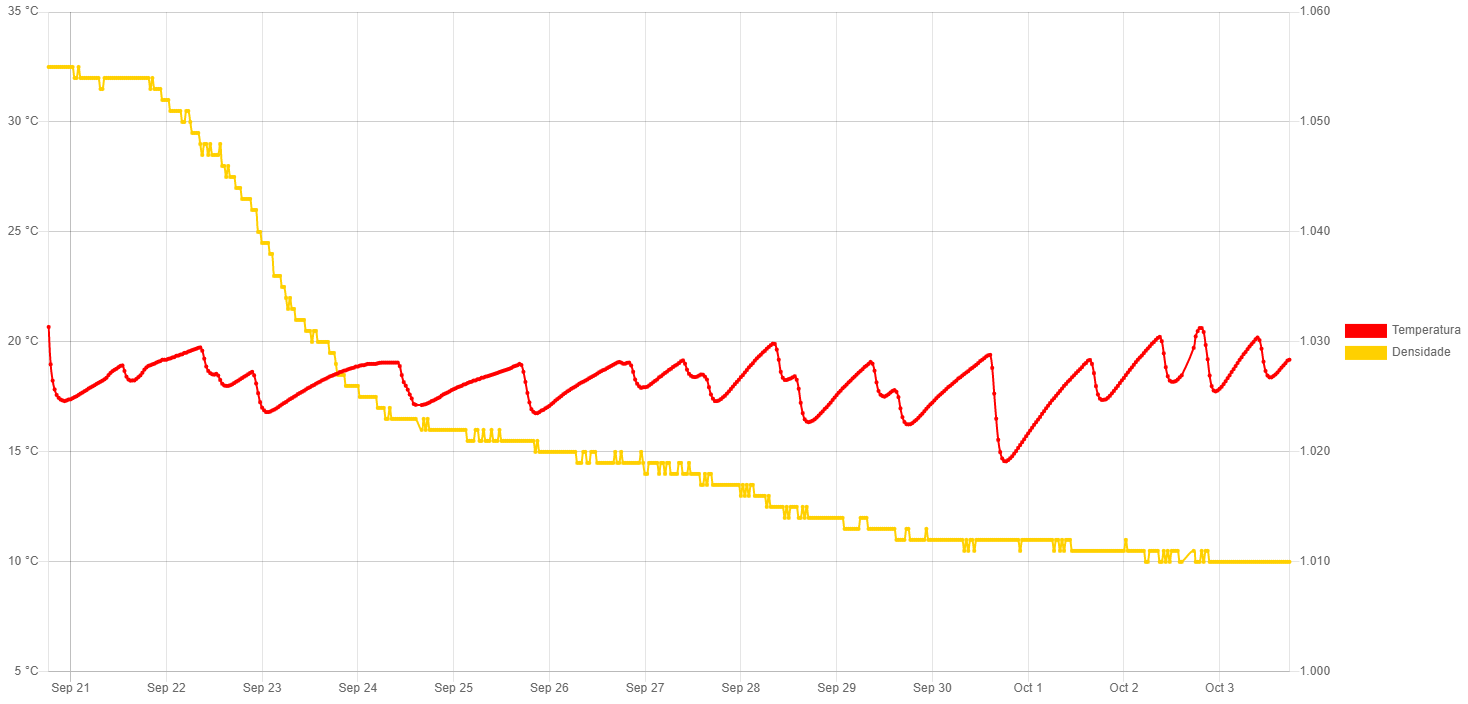
\includegraphics[scale=0.4]{figuras/implementacao/software/grafico_chartjs.PNG}
    \caption{Exemplo de gráfico de evolução das variáveis.}
    \label{fig:grafico_chart}
\end{figure}


\subsection{Implantação}


A partir dos containers que definidos por cada aplicação de backend, a implantação de todos os sistemas podem ser orquestrados em um único comando utilizando a ferramenta Docker Compose definindo uma aplicação multi-container. Existem hoje tecnologias mais robustas como o Kubernetes para fazer o provisionamento e monitoramento de vários containers, mas o Docker Compose foi escolhido pela sua simplicidade. Dessa forma, os serviços backend e o broker de mensagens MQTT são provisionados em uma máquina virtual oferecida pelo serviço de computação em nuvem AWS.o


A configuração dos serviços é feita de forma que apenas o broker e o Servidor de Aplicação estejam expostos a acesso externo, protegendo os demais serviços. Essa configuração pode ser conferida no arquivo \textit{docker-compose.yaml} no repositório de código: \url{https://github.com/josehcls/tcc-config}.


A Interface Web foi provisionada pela plataforma Vercel, que oferece o serviço de hospedagem gratuito, sob condições, e algumas facilidades como construir e disponibilizar o acesso à plataforma web a partir do código no repositório do GitHub.

